\documentclass[a4paper,12pt]{article}
\usepackage[T1]{fontenc}
\usepackage[utf8]{inputenc}
\usepackage{graphicx}
\usepackage{amsmath}
\numberwithin{equation}{subsection}
\newcommand*{\myTitle}{\begingroup 
\centering 
\vspace*{\baselineskip} 
{\LARGE Mössbauer-effektus vizsgálata(MOS)}% Title
\vspace*{1\baselineskip}

\scshape % Small caps
Korszerű Vizsgálati Módszerek Laboratórium

\vspace*{1\baselineskip}
Eötvös Lóránd Tudományegyetem\\[\baselineskip]
Természet Tudományi Szak\\[\baselineskip]
Fizika Bsc\\[\baselineskip]
\vspace*{5\baselineskip} 
Szerző\\[\baselineskip]
{\Large Máthé Marcell Tibor\par} 
\vspace*{3\baselineskip}
Mérőtársak \\
{ Katona Dávid, Olár Aley \par} 

\vspace*{1\baselineskip}
\today

\endgroup\clearpage}

 \renewcommand{\contentsname}{\underline{Tartalomjegyzék}}
\renewcommand{\refname}{Irodalomjegyzék}

\begin{document}
\thispagestyle{empty} 
\myTitle
\newpage
\thispagestyle{empty}
\tableofcontents
\newpage
\section{Bevezetés}
Az alábbi jegyzőkönyvben a ELTE-Korszerű vizsgálati módszerek laboratórium keretein belül elvégzett Mössbauer-effektus vizsgálata(MOS) című mérés eredményeit és az abból levont következtetéseimet mutatom be.A mérést a -1.111, Korecz László Laboratóriumban végeztük a mérő társaimmal. Az effektus részletes elméleti tárgyalása a \\ http://atomfizika.elte.hu/kvml/docs/korszeruosszefuzott.pdf címen a 12. fejezetben a 251. oldaltól megtalálható. 
\subsection{Mérés célja}
Különböző anyagok Mössbauer- spektrumának felvétele (lágyvas,rozsdamentes acél, nátrium-nitroprusszid). Illetve ezek által becslést adni a mag mágneses nyomatéknak a mágneses térrel való kölcsönhatás okozta felhasadásra illetve a kvadrupól momentumnak az inhomogén elektromágneses térrel való kölcsönhatásából eredő felhasadásra, majd ezeket összehasonlítani az elméletekből eredő mennyiségekkel.
\subsection{Mérés rövid leírása}
A mérés során a fotonokat kibocsátó forrást egy hangfalra rögzítve mozgattuk állandó gyorsulás mellett (a sebesség idő grafikon egy háromszög jel) és így a Doppler-effektust felhasználva végig lehet pásztázni a kívánt energia tartományt. \[\Delta E=E_{\gamma}\frac{v}{c}\]  A bejövő fotonokat egy proporcionális számlálóval detektáljuk majd ezt a jelet különböző szűrőkön átvezetve egy sokcsatornás analizátorra vezetjük. Forrásnak egy $^{57}$Co- et használunk mely atomok egy elektron befogás után $^{57}$Fe-vé alakulnak át, amik a legerjesztődés során 91\% valószínűséggel egy 14,4KeV energiájú fotont bocsát ki. Ez az energia a mérés szemszögéből is hasznos mert proporcionális kamra hatáskeresztmetszete a kisebb energiájú fotonokra nagyobb, illetve a létrejövő $^{57}$Fe élettartama viszonylag nagy emiatt a kibocsátott foton vonalszélessége kicsi. A már fentebb említett szűrőkkel a berendezést erre az energiára állíthatjuk rá, ezt a mérés kezdeténél nekünk kellett beállítani. Eztán a lágyvas,rozsdamentes acél és a nátrium-nitroprusszid mintákat kellett a berendezésbe behelyezni, a bejövő jeleket egy DOS-os szoftverrel elemeztük. Mivel a hangfal sebessége egy perióduson belül kétszer ugyan az így az ábrákon is minden esetben párosával jelentek meg a csúcsok, ezt a szoftver segítségével félbe hajtva tovább lehetett csökkenteni a jel-zaj arányt, majd ugyanezzel a programmal különböző fajtájú Lorentz-görbéket illesztettünk az adatokra.
\newpage
\section{Mért adatok és kiértékelésük}
\subsection{Kalibrálás}
Mivel a forrás sebessége a hangszóróra erősítve lineárisan változik az időben így a csatornaszám-energia függvény is lineáris lesz, továbbá mivel csak energiakülönbségeket tudunk ezzel a módszerrel mérni így a kalibráláshoz elegendő a kalibrációs egyenes meredeksége. Felhasználva hogy a lágyvas két legtávolabbi csúcsúnak távolsága Doppler-sebességben $d_v=10.6162$ (Ez irodalmi érték). A mérés alapján pedig a két csúcs távolsága $d_{cs}=366.61\pm 0.957$. Ezeket az adatokat felhasználva a meredekség.
\[m=E\frac{d_v}{d_{cs}c}=(1.3909 \pm 0.00036)\cdot10^{-9} eV\]
\begin{figure}[h!]
\centering
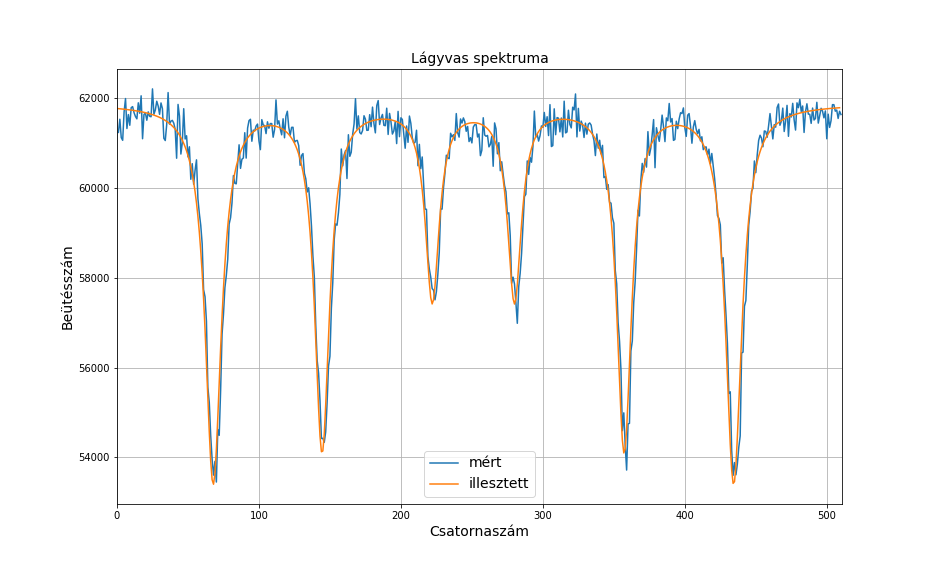
\includegraphics[width=12cm]{vas.png}
\caption{A kalibráláshoz a két legszélső csúcs csatornaszámbeli különbségét használjuk fel}
\end{figure}
\subsection{A rozsdamentes acél és a nátrium-nitroprusszid minta izomér eltolódása a lágyvashoz képest}
A magnak az elektronfelhővel való elektrosztatikus kölcsönhatása kis mértékben módosítja a mag energiaszintjeit ezt nevezik izomér eltolódásnak, az eltolódás mértéke jellemezhető a Mössbauer-spektrummal és így meghatározható a minta szerkezete és anyagösszetétele. Az effektus során a rozsdamentes acélban és nátrium-nitroprusszidban megtalálható vasmagok eltolódását vetjük össze a lágyvaséval. Érdemes megjegyezni hogy izomér eltolódást sok egyéb effektus is okozhat(pl gravitációs tér, kristályszerkezeti elváltozások) de ezektől itt most eltekintünk.
A lágyvashoz tartozó spektrumban a Zeeman-felhasadás miatt 6 db csúcs van (Lsd.: 1 ábra) a nívók eredeti helyét úgy becsülhetjük meg hogy az illesztés során olyan Lorentz-görbéket illesztünk az adatokra, hogy a csúcsokat párokba rendezzük majd egy (felhasadás nélküli) helyhez képest tekintjük a távolságukat, így minden görbe párhoz 4 db adat tartozik ezek az alábbi táblázatban láthatóak 
\begin{table}[h!]
\centering
\begin{tabular}{|c|c|}
\hline
		alapvonal ($B$) & $61883 \pm 22 $\\
		\hline
		1. amplitúdó ($A_1$) & $8418 \pm 83 $\\
		\hline
		1. csúcs helye (felhasadás nélkül) ($x_{0, 1}$) & $252.09 \pm 0.07$\\
		\hline
		1. csúcs szélessége ($\Gamma_1$) & $13.86 \pm 0.2$\\
		\hline
		1. felhasadás ($S_1$) & $366.6 \pm 0.1$ \\
		\hline
		2. amplitúdó ($A_2$) & $7682 \pm 86 $\\
		\hline
		2. csúcs helye (felhasadás nélkül) ($x_{0, 2}$) & $251.86\pm 0.07$\\
		\hline
		2. csúcs szélessége ($\Gamma_2$) & $12.62 \pm 0.2 $\\
		\hline
		2. felhasadás ($S_2$) & $212.8 \pm 0.1$ \\
		\hline
		3. amplitúdó ($A_3$) & $4327 \pm 89 $\\
		\hline
		3. csúcs helye (felhasadás nélkül) ($x_{0, 3}$) & $252.06 \pm 0.12$\\
		\hline
		3. csúcs szélessége ($\Gamma_3$) & $11.89 \pm 0.4$\\
		\hline
		3. felhasadás ($S_3$) & $57.92 \pm 0.24$ \\
		\hline

\end{tabular}
\caption{A lágyvas spektrumára illesztett Lorentz görbék paraméterei}
\end{table}
A három felhasadás nélküli csúcs helyet kiátlagolva kaphatjuk meg a Zeemann-effektus nélküli helyet.
\[IS_{lv}=\frac{252.09+251.86+252.06}{3}=252.0 \pm0.05 \]
ezután ugyan ezt az illesztési módszert elvégezve az acélra és nátrium-nitroprusszid-ra
\newpage
\begin{table}[h!]
\centering
\begin{tabular}{|c|c|}

		\multicolumn{2}{c}{Rozsdamentes acél} \\
		\hline
		alapvonal ($B$) & $1170.6 \pm 1.7 $\\
		\hline
		amplitúdó ($A$) & $342.0 \pm 13.3 $\\
		\hline
		csúcs helye ($x_0$) & $247.65 \pm 0.32$\\
		\hline
		szélesség ($\Gamma$) & $16.57 \pm 0.96$\\
		\hline

		\hline
		\multicolumn{2}{c}{Nitroprusszid-nátrium} \\
		\hline
		alapvonal ($B$) & $2631.9 \pm 2.6 $\\
		\hline
		amplitúdó ($A$) & $364.5 \pm 18.7 $\\
		\hline
		csúcs helye (felhasadás nélkül) ($x_0$) & $242.55 \pm 0.25$\\
		\hline
		szélesség ($\Gamma$) & $9.86 \pm 0.73$\\
		\hline
		felhasadás ($S$) & $59.51 \pm 0.50$ \\
		\hline

\end{tabular}
\caption{A spektrumra illesztett Lorentz görbék paraméterei}
\end{table}

 Az illesztések alapján az izomér eltolódásokra különböző anyagokra:
\begin{table}[h!]
\centering
\begin{tabular}{c||c|c}
lágyvas&$252\pm0.05$& 0\\
rozsdamentes acél&$247.65\pm0.32$&$(6.0504\pm0.0094)\cdot10^{-9} eV$ \\
nátrium-nitroprusszid&$242.55\pm0.25$&$(1.3144\pm0.0017)\cdot10^{-8}eV$ \\
\end{tabular}
\end{table}
\\
ahol táblázat harmadik sorában az első alfejezetben használt kalibrációs meredekséget használtuk fel \[\Delta E_{ab}=m*(SI_a-SI_b)\]módon. 
\subsection{A gerjesztett állapot élettartama és a minták vastagsága}
A jegyzetben a 261.o (12.11) képlete alapján a valódi vonalszélesség
\[\frac{\Gamma_{mert}}{\Gamma}=2+\frac{\omega_iT_A+T_F}{4}-\frac{(\omega_iT_A+T_F)^2}{625}\] ahol $T_A$ az abszorbens (itt lágyvas) $T_F$ pedig a forrás vastagsága $\omega_i$ pedig az i-edik felhasadás relatív intenzitása. Lágy vas esetén ez 
\begin{table}[h!]
\centering
\begin{tabular}{c c c}
Ámenet&Arány&$\omega_i$ \\ \hline
$\pm \frac{3}{2}\leftarrow\pm\frac{1}{2}$& : 3 &1/4\\
$\pm \frac{1}{2}\leftarrow\pm\frac{1}{2}$& : 2&1/6\\
$\pm \frac{3}{2}\leftarrow\mp\frac{1}{2}$& : 1&1/12\\

\end{tabular}
\end{table}
Ha a fenti képletből a másodrendű tagokat elhanyagoljuk és felhasználjuk hogy $T_F=1.62$ akkor a következő lineáris összefüggésre jutunk
\[\Gamma_{mert}=2.4\Gamma+\frac{1}{4}T_A\omega_i\Gamma\]
Az 1.Táblázatból a vonalszélességeket ábrázolva a relatív intenzitások függvényében:
\begin{figure}[h!]
\centering
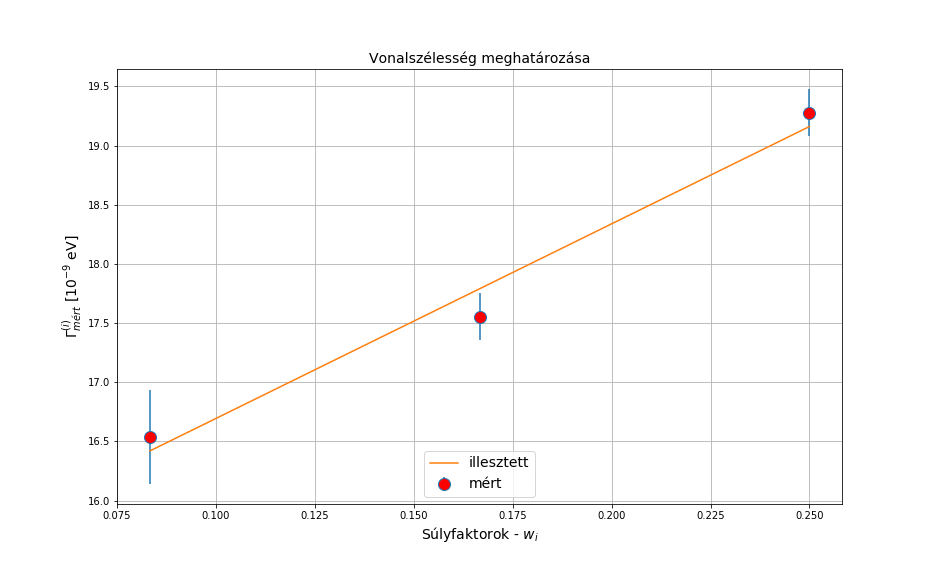
\includegraphics[width=12cm]{vonalszelesseg.png}
\end{figure}
\\ ahol az illesztett egyenes egyenlete: \[f(x)=(16.441\pm2.457)\cdot x+15.050\pm0.442\] ami alapján a \[\Gamma=(6.271\pm 0.184)\cdot10^{-9} eV\] \[\tau=\frac{\hbar}{\Gamma}=(1.052\pm 0.031)\cdot10^{-07} s\]
azaz a mért $\tau_{mert}=105.2\pm3.1 ns$ míg az irodalmi érték pedig $\tau_{irod}=141.8ns$ ami jelentős eltérés.
A minták relatív vastagságát szintén a fenti illesztésből lehet megkapni \[T_A=\frac{4\cdot (16.441\pm2.457)}{\Gamma_{cs}}=14.586\pm2.608\] ahol $\Gamma_{cs}$ a csatornaszámbeli érték, hogy a vastagság egy dimenziótlan szám legyen. A többi mintára ez a vastagság a fenti képlet átrendezéséből \[T_A=\left(4\frac{\Gamma_i}{\Gamma}-T_F-8\right)\frac{1}{\omega_i}\] így a rozsdamentes acél és a nátrium-nitroprusszid vastagsága:
\[T_{ac}=5.081\pm0.444\]
\[T_{nn}=-0.872\pm0.1\] a nátrium-nitroprusszidra kapott adat nyilvánvalóan fizikai ellentmondás.
Annak hogy a másodrendű tag elhagyása mekkora mértékben módosítaná a kapott eredményeket, az elhagyott tag értéke a lágyvasra a fenti adatokkal és $\omega=1/4$ $\delta=0.013$ tehát csak a második tizedes jegyben okozna eltérést ami elhanyagolható.
\subsection{Az elektromos térgradiens a nátrium-nitroprusszid mintában}
A nátrium-nitroprusszidban az atomok elrendezéséből eredendően inhomogén elektromos tér alakul ki ami a mag kvadrupól momentumával kölcsönhatva a magnívók felhasadásához vezet. A felhasadás mértéke a jegyzet alapján \[\Delta E=\frac{eQ}{4I(2I-q)}\frac{\partial^2 V}{\partial z^2}\left(3m^2_I-I(I+1\right)\sqrt{1+\frac{\eta^2}{3}}\] ahol $Q$ az atommag kvadrupól momentuma (itt $Q_{3/2}=0.21\cdot10^{-28}m^2$), $e$ az elemi töltés, $I$ a magnívó spinje(itt $I=3/2$) $m_i$ a mag mágneses kvantumszáma (itt $m_i=\pm3/2, \pm1/2$), $\eta$ pedig az asszimmetria faktor mely esetünkben 0. Mivel a képletben az $m_i$ a négyzetre van emelve így az energiaszint csak kettő részre hasad fel, ezen két szint távolsága
\[\Delta E=\frac{eQ}{2} \frac{\partial^2 V}{\partial z^2}\], a mérésein alapján ez a $\Delta E_m$ a Lorentz illesztésből megkapható
\[\Delta E_m=m*59.51=(8.277\pm0.716)10^{-9}eV\]
amiből a fenti egyenlet segítségével a térgradiens értéke megkapható 
\[\frac{\partial^2 V}{\partial z^2}=(7.883 \pm 0.069)\cdot10^{21} V/m^2\]
Összehasonlítás ként a hidrogénatom Bhor-modelljében az alapállapotú elektron által a proton helyén létrehozott elektromos térgradiense( amit a Coulomb potenciált kétszeri deriválásával kapunk)  \[\frac{\partial^2 V}{\partial z^2} \bigg\vert_{elm}=\frac{1}{2\pi\epsilon_0}\frac{r}{r^3_B}=1.95\cdot10^{22}\frac{V}{m^2}\] a mért és az elméleti adatok majdnem egy nagyságrendbe esnek.
 \subsection{Az $^{57}Fe$ mágneses momentuma a első gerjesztett állapotban és a B értéke a lágyvas mintában}
A mágneses kvantumszám szerint degenerált nívók felhasadás külső mágneses térben a Zeeman-effektus, a felhasadás mértékét pedig a \[\Delta E_m=-\frac{m_I}{I}\mu_IB\] használjuk fel a (2.3) as fejezetben meghatározott relatív intenzitásokat az átmeneteket és határozzuk meg hozzájuk paraméteresen az energiák értékeit(A,B,C paraméterekkel)
\begin{figure}[h!]
\centering
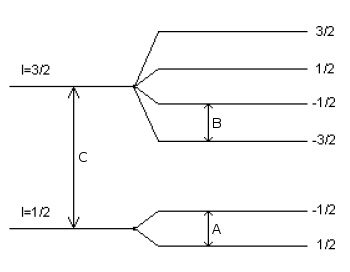
\includegraphics[width=8cm]{atmenet.png}
\caption{A felhasadt energia nívók szerkezete}
\end{figure}
\begin{table}[h!]
\centering
\begin{tabular}{c c}
Ámenet& Energia értékek paraméterekkel \\ \hline
$\pm \frac{3}{2}\leftarrow\pm\frac{1}{2}$& A+3C\\
$\pm \frac{1}{2}\leftarrow\pm\frac{1}{2}$& A+C\\
$\pm \frac{3}{2}\leftarrow\mp\frac{1}{2}$& A-C\\
\end{tabular}
\end{table}
Isteni sugallatból azaz az előző évek jegyzőkönyveit alaposan tanulmányozva megállapítható hogy a legpontosabb illesztés abban az esetben lehet tenni az adatokra ha a C függvényében (3C,1C,-1C) ábrázoljuk az adatokat és azokra egyenest illesztünk (ahol N=(3,1,-1))
\[N=C\cdot \Delta E+A\]  ahol $\Delta E$ a lágyvashoz tartozó energiaszintek felhasadásának mértéke
\begin{table}[h!]
\centering
\begin{tabular}{c c}
Átmenet & Energiaszint($10^{-9}eV$)\\ \hline
$\Delta E_1$=A+3C& $509.90\pm0.19$\\
$\Delta E_1$=A+C& $295.98\pm0.16$\\
$\Delta E_1$=A-C& $80.56\pm0.33$\\
\end{tabular}
\end{table}
\newpage
ha ezeket az adatokat az előző képlet alapján ábrázoljuk. 
\begin{figure}[h!]
\centering
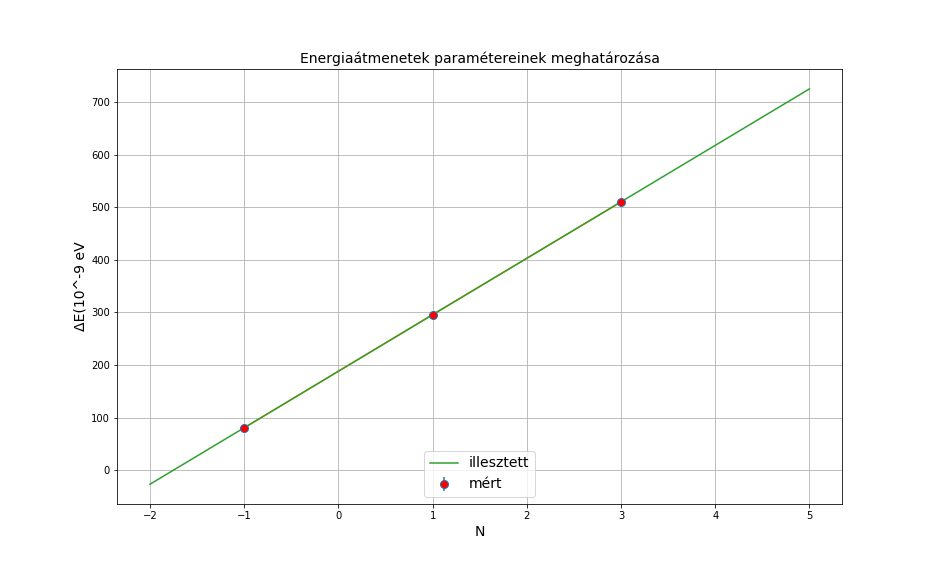
\includegraphics[width=12cm]{parameterek.png}
\end{figure}
\\Az illesztett egyenes paraméterei 
\begin{table}[h!]
\centering
\begin{tabular}{c c}
$A=(188.145 \pm 0.414)\cdot 10^{-9} eV$ & $C=(107.335\pm0.216)\cdot 10^{-9}eV$
\end{tabular}
\end{table}
\\a jegyzet alapján a mag mágneses momentuma alapállapotban $\mu_{1/2}=0, 090604 \mu_N$ illetve $\mu_N=3, 15238\cdot 10^{-11} \frac{keV}{T}$ használjuk fel hogy az alapállapotban \[\Delta E=\frac{\mu_{1/2}B}{I_{1/2}}=A \] és a gerjesztett állapotban
\[\Delta E=\frac{\mu_{3/2}B}{I_{3/2}}=-C\]
ha a két egyenletet elosztjuk egymással akkor abból a $\mu_{3/2}$ meghatározható
\[\mu_{3/2}=-\frac{I_{3/2}}{I_{1/2}}\mu_{1/2}\frac{C}{A}=(-5.43\pm0.13)\cdot 10^{-12}\frac{keV}{T}\] illetve az illesztett paraméterek segítségével kiszámolható a maghelyén lévő mágneses indukció
\[B=\frac{I_{1/2}}{\mu_{1/2}}A=(32.936\pm0.07) T\]
Ezt az értéket is érdemes összevetni az elektron által keltett mágneses térrel a meg helyén, ezt az értéket a \[B_m=\frac{\mu_0\hbar e }{m_e 4 \pi r^3_b} \] képlet adja meg aminek számszerű éréke \[B_m=12.5T\] az általunk mért érték ennek közel a három szorosa.
\subsection{A forrás és a minta távolságából eredő lehetséges hiba}
A méréssorán végig felhasználtuk azt a tényt hogy a forrás és a minta közti távolság végig $\sim 1 cm$ marad ami persze nem igaz hiszen a mérés pont abból ered hogy a forrást mozgatjuk a kérdés, hogy mekkora a távolság különbségből eredő hiba. A hangszóróra adott jel alakjából tudjuk hogy a sebesség a a periódus feléig nő utána pedig csökken. A periódus idő a jegyzet alapján $T_p=41.2\pm2ms$ az első alfejezetben számolt kalibrációs meredekséggel meglehet becsülni a maximális sebességet is.  \[v_{max}=c\frac{\Delta E_{256}}{E_0}\] ahol $E_{256}$ a 256-os csatornának megfelelő energia szint ami a T/4-hez tartozó csatornaszám. \[v_{max}=(7.418\pm0.002)\frac{mm}{s}\] ez alapján a maximális kitérés \[d_{max}=v_{max}\frac{T}{4}=(0.0764\pm0.004) mm \] azaz a maximális kitérés sem éri el az egytized millimétert tehát kijelenthető hogy ez a járulék elhanyagolható a mérés során.
\subsection{A gravitációs vöröseltolódás kimérése}
Ennek a módszernek a hihetetlen pontosságát az is mutatja hogy Pound és Rebka 1960-ban ezt az effektust kihasználva már 20m távon kitudta mutatni a gravitációs vörös eltolódást. Érdemes kiszámolni hogy a laborba található eszközzel ennek a kiméréséhez milyen magasságra van szükség. \\A földről indított $E_f=14.4keV$ energiájú fotonnak meg kell másznia a föld által létrehozott gravitációs potenciált $\Phi=mgh$ és ezalatt a foton energiát veszít és így eltolódik a vörös felé. A laborban található eszköz pontossága 0.5 csatorna ezt átszámíthatjuk energiára $(E_l=6.95\cdot10^{-10}eV)$-nak felel meg, azaz ha ennyit változik a foton energiája azt már ki lehet mérni az eddig is használt eszközzel. Ebből az energiából a magasságra \[h=\frac{E_l}{E_f}\frac{c^2}{g}=442.78\] ilyen magasságra kéne tenni a detektort hogy az effektus kimérhető legyen. A mérést tovább bonyolítja hogy minél magasabban van a detektor annál kisebb térszög lesz a területe és így jelentősen tovább is tartana a mérés, illetve a fotonoknak amíg felérnek nem szabad hogy energiát adjanak le a köztes atomoknak így vagy egy vákuum csőben vagy speciális gázzal feltöltött csőben kéne a fotonokat a detektorig vezetni.
\end{document}

